%%%%%%%%%%%%%%%%%%%%%%%%%%%%%%%%%%%%%%%%%%%%%%%%%%%%%%%%%%%%%%%%%%%%%%%%%%%%%%%%
%2345678901234567890123456789012345678901234567890123456789012345678901234567890
%        1         2         3         4         5         6         7         8

\documentclass[letterpaper, 11 pt, conference]{ieeeconf}  % Comment this line out
                                                          % if you need a4paper
%\documentclass[a4paper, 10pt, conference]{ieeeconf}      % Use this line for a4
                                                          % paper

\IEEEoverridecommandlockouts                              % This command is only
                                                          % needed if you want to
                                                          % use the \thanks command
\overrideIEEEmargins
\usepackage{url}
\usepackage{graphicx}

% See the \addtolength command later in the file to balance the column lengths
% on the last page of the document



% The following packages can be found on http:\\www.ctan.org
%\usepackage{graphics} % for pdf, bitmapped graphics files
%\usepackage{epsfig} % for postscript graphics files
%\usepackage{mathptmx} % assumes new font selection scheme installed
%\usepackage{times} % assumes new font selection scheme installed
%\usepackage{amsmath} % assumes amsmath package installed
%\usepackage{amssymb}  % assumes amsmath package installed

\title{\LARGE \bf
Design and Implementation of a Scalable Distributed Graph Database
}

%\author{ \parbox{3 in}{\centering Huibert Kwakernaak*
%         \thanks{*Use the $\backslash$thanks command to put information here}\\
%         Faculty of Electrical Engineering, Mathematics and Computer Science\\
%         University of Twente\\
%         7500 AE Enschede, The Netherlands\\
%         {\tt\small h.kwakernaak@autsubmit.com}}
%         \hspace*{ 0.5 in}
%         \parbox{3 in}{ \centering Pradeep Misra**
%         \thanks{**The footnote marks may be inserted manually}\\
%        Department of Electrical Engineering \\
%         Wright State University\\
%         Dayton, OH 45435, USA\\
%         {\tt\small pmisra@cs.wright.edu}}
%}

\author{Ashrith Sheshan, Aakash Arayambeth, Jayanth Kalyanasundaram % <-this % stops a space
}


\begin{document}



\maketitle
\thispagestyle{empty}
\pagestyle{empty}


%%%%%%%%%%%%%%%%%%%%%%%%%%%%%%%%%%%%%%%%%%%%%%%%%%%%%%%%%%%%%%%%%%%%%%%%%%%%%%%%


%%%%%%%%%%%%%%%%%%%%%%%%%%%%%%%%%%%%%%%%%%%%%%%%%%%%%%%%%%%%%%%%%%%%%%%%%%%%%%%%
\section{INTRODUCTION}
Today, there are a breadth of applications that process highly connected data by exploiting the connectivity and relationship between bits of information. Social Networking, recommendations based on relationships, Knowledge graphs to improve information retrieval, fraud detection etc are a few use cases for highly connected data.\\
 Using relational databases to build such applications poses a few challanges. SQL is not designed to process relationships well. As the number of relationships grows, the SQL query becomes quite complicated and suffers from performance issues. With highly connected data, the types of information that need to be processed change rapidly. This requires the database system to be flexible to accommodate new data types. Relational Databases don't evolve their schema very well; they are relatively inflexible. \\
 On the other hand, Graph databases are optimized for efficient storage and retrieval of highly connected data and are hence, key to building applications that look to leverage connectivity among bits of information. The need for a distributed, fault-tolerant, scalable graph database is imminent. However, designing a distributed and sharded graph database has proved to be a challenging task due to lack of record-wise separation and strong connections in graph data. Hence, we plan to design a distributed, fault tolerant graph database while exploring the intricacies of storing and querying graph data.


\section{RELATED WORK}
  
 In recent times, many graph databases have evolved and become prominent, but the fact that big players like Amazon releasing NeptuneDB\cite{neptunedb} in late 2017 and Microsoft releasing CosmosDB\cite{cosmosdb} in mid 2017 with not so significant market share for distributed graph database proves that this field is still naive. AWS' NeptuneDB\cite{neptunedb} is cloud-native database application on AWS. Though AWS claims high scalability, its performance is not comparable to single server graph databases such as Neo4j\cite{neo4j} as ranked by \cite{dbranking}. After evaluating the architecture, we suspect that it is because the database application layer is not aware of the distributed nature of the underlying storage and uses the AWS S3 storage abstraction. We believe that knowledge of data locality is important from the database's perspective for its best performance.\\
 
 Trinity\cite{trinity} is a distributed graph engine on a memory cloud. It implements a globally addressable distributed memory storage that is used to store the graph topology and other critical information. The richer information is stored on disk. The distributed memory storage is divided into memory trunks and graph vertices are stored as key-value pairs and hashed into one of these memory trunks. The trunks are replicated onto multiple servers and operations on them are considered committed only when they are stored to a distributed filesystem. Failures of nodes are handled by syncing from the distributed filesystem.\\
 
 SystemG\cite{systemg} uses the Apache TinkerPop interface to  implement a graph storage on top of four distributed key value stores. Two for storing vertices with the properties, one for storing edges from source to destination and one from destination to source along with the edge properties. Consistent hashing is used to distribute vertices among nodes, and edges are always stored on the node that contains the source vertex. The paper discusses ways to optimize batched insertions of large numbers of vertices/edges in a graph. It also implements a query manager to efficiently process complex graph queries.\\ 
 
 GraphChi\cite{graphchi} introduces Parallel adjacency lists - a data structure that can store graphs compactly on disk while simultaneously enabling fast access to both incoming and outgoing edges, without duplicating data.\\
 
 G-Store\cite{g-store} strategically places data on pages so that time needed for graph specific access patterns is minimized. It tries to place nearby vertices on pages that are closer and have minimum access overhead. 




\section{DESIGN}
%For our evaluation we intend to create different scenarios of network overheads in a containerized application and benchmark the network performance on metrics like and bandwidth

We build a distributed database designed to store graph data with the following requirements: \\
\begin{enumerate}
\item \textit{Consistent} - Graph traversals from multiple vertices which may reside in different machines should still result in the seeing the same graph structure and properties at any point of time.
\item \textit{Fault tolerant and Replicated} - System will sustain node failures at all times.
\item \textit{Sharded} - Not all graph data is replicated everywhere. This can also be extended to geo-local sharding to improve data locality based on query analytics \\
\end{enumerate} 

We implement the Apache Tinkerpop\cite{tinkerpop} graph query interface with our graph engine backing the data store. We use existing Key Value stores such as Zookeeper or Cassandra to store metadata about the system. Fig.\ref{fig:arch} shows a rough estimate of the particulars we design and implement. The components marked in grey were designed and implemented as part of this project. The remaining parts were leveraged from existing open source solutions. \\
We offload DB client management tasks to using a fault tolerant gateway like nginx which could reside on top of our default gateway to provide IP failover for clients. We will also provide approximate performance constraints for which the system is designed.\\
\begin{figure}
 \centering
  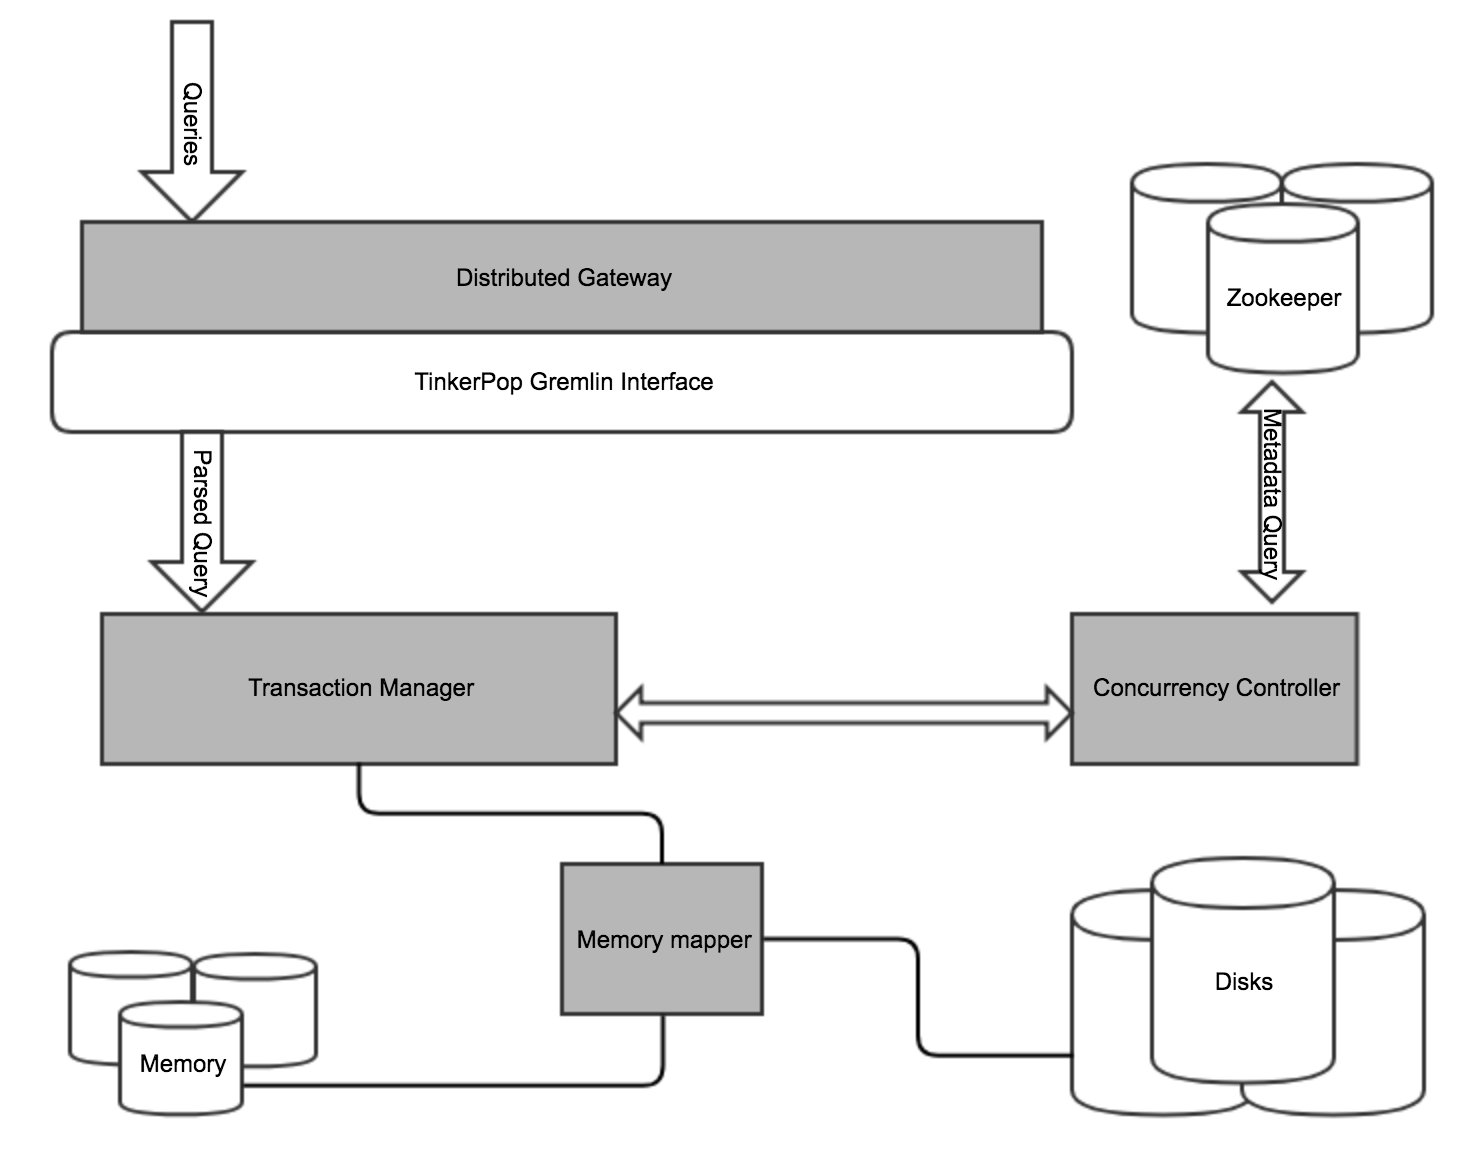
\includegraphics[width=0.5\textwidth]{arch.png}
\caption{Architecture Design}
\label{fig:arch}
\end{figure}

Based on the evaluations and our design, we intend to answer the following questions:
\begin{enumerate}
	\item How can graphical data be stored - vertices and edges?
    \item How to traverse a graph stored on disk? Do we cache the graph structure on RAM or is there a better way?
	\item How to shard the nodes of a big connected graph across nodes which optimizes queries?
    \item How different is it to handle replication of graphical data for improved fault tolerance? 
\end{enumerate}

\section{FEATURE DESIGN}
\begin{enumerate}
	\item \textbf{Scalability: } 
As more servers are added, our system scales on writes without significant loss in performance. Partitioning enables write operations to different parts of the graphs to execute concurrently. Adding more servers enables us to house more partitions , thereby increasing concurrency. Additionally, increasing the number of servers enables the system to service larger graphs. 
After evaluating the proposed system’s performance, we leave open an option to allow reads to happen from replicas (with the help of transaction IDs) to achieve improved performance at scale. \\
	\item \textbf{Consistency Model:} 
Our system guarantees causal consistency. Which means that when a client reads from this database, it is assured to read at least it's own writes that have been acknowledged by the system. The guarantee is that the client will always see it’s most recent write when it reads.\\
We do not strive to achieve sequential consistency. While we do ensure that a single client’s requests are serviced in program order, we do not enforce an arbitrary total order across all replicas or shards. If two clients write to two different parts of the graph, residing in different shards, then there is no need to  ensure a total order of execution of these two writes across all replicas. We leave scope to move from a causally consistent model to an eventually consistent model, should the former prove to be a performance bottleneck. \\
	\item \textbf{Fault Tolerance}
    We achieve fault tolerance by replicating graph partitions and coordinating client interactions with partition replicas. The number of failures that our system tolerates and consequently, the number of replicas required, will be determined by a user-defined replication factor. We operate under the assumption that the replicas experience only random independent failures such as memory errors or hard-drive crash.\\
    
 \item \textbf{Partitioning scheme: }
 \begin{figure}
 \centering
  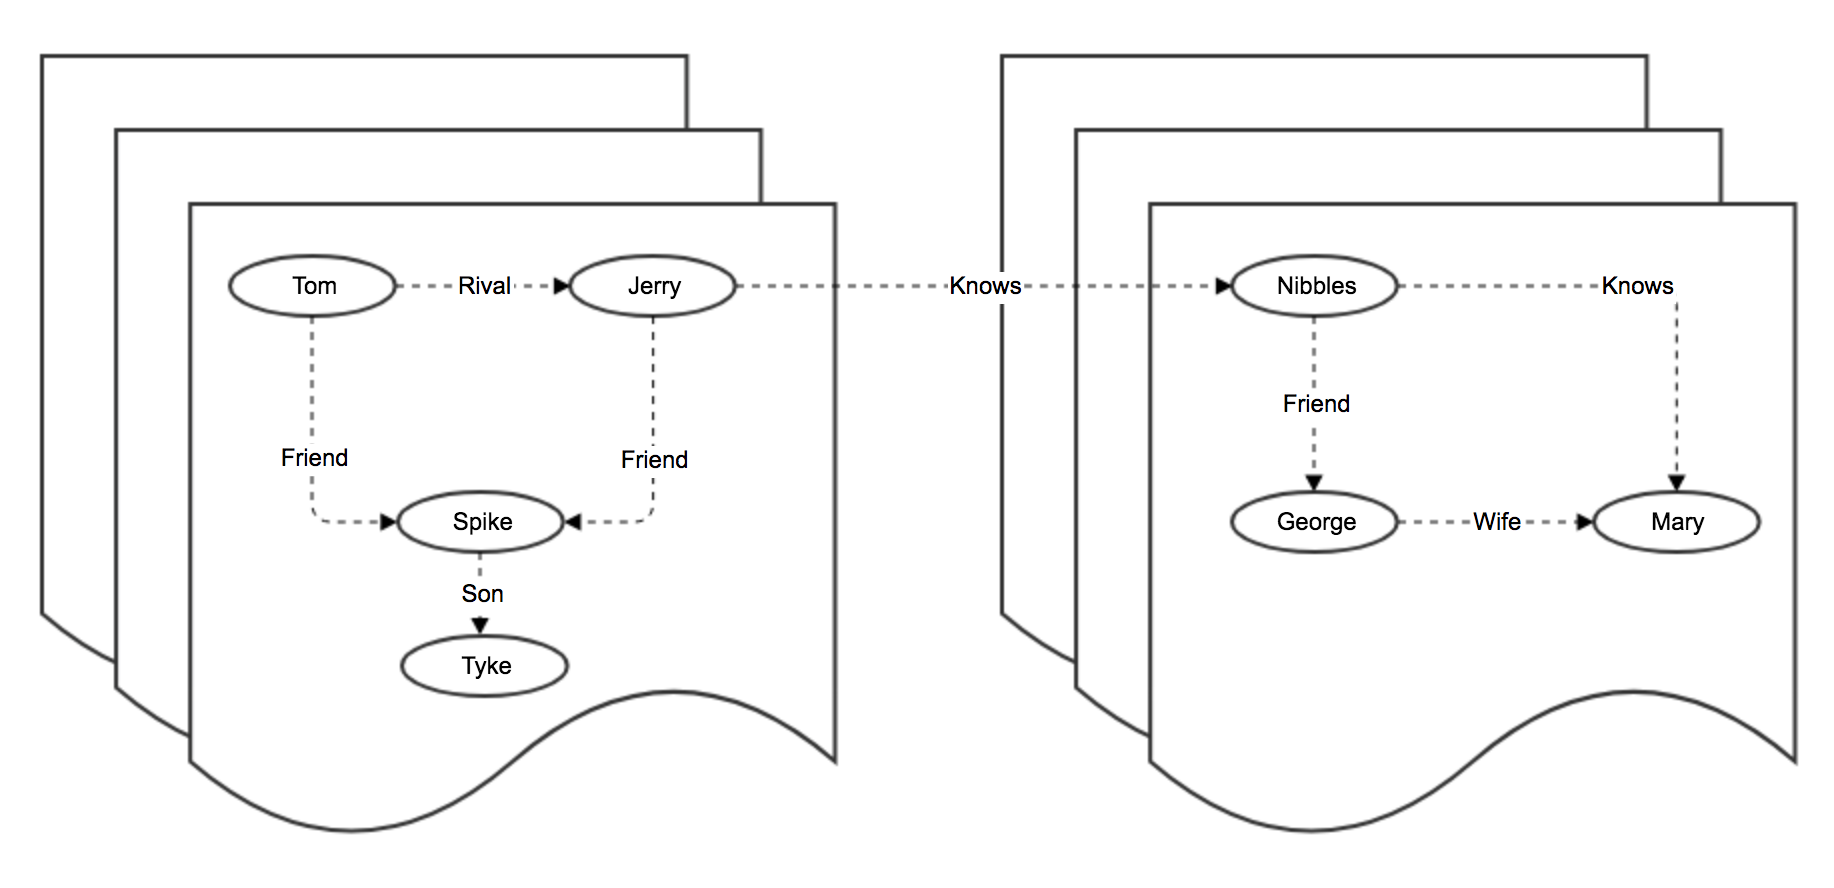
\includegraphics[width=0.5\textwidth]{replicas.png}
\caption{Partitioning of the graph}
\label{fig:rep}
\end{figure}
Graph data can be terabytes to petabytes in size. Storage of such large data requires a distributed system, but special attention must be paid to the structure of the graph when it comes to partitioning the graph across a cluster of servers. Graph based queries in general, have the property of traversing from a small set of nodes to their neighbors, to their neighbors’ neighbors etc. Hence, keeping closely colocated vertices and edges stored on the same partition allows us to reduce the amount of network communication required to perform these traversal queries. Many partitioning schemes have been proposed for large graph based datasets. We draw inspiration from the multilevel partitioning scheme mentioned in G-Store\cite{g-store} for our distributed graph store. Vertices and edges are stored in storage backends such that the following costs are minimized:
\begin{enumerate}
\item Cost of placing adjacent vertices on different machines in the system. This cost is reduced by placing a group of highly connected adjacent vertices on the same machine.
\item Cost of number of edges across machines. Greater the number of edges across the machines, greater the cost
\item Cost of number of linked machines. More number of linked machines, the cost of graph traversal increases
\end{enumerate}
These costs together give us an optimization problem which tries to keep strongly connected vertices on the same partition while separating weakly connected components onto different partitions. We focus primarily on costs $(a)$ and $(b)$ and use the heavy edge matching algorithm mentioned in the paper to create a coarsened graph of compound vertices that serve as the partitions. A significant difference between what we solve and what was solved in G-Store is that different partitions are stored on different servers while in G-Store, different partitions are stored on different disk pages of the same machine. Another difference is that we need to run the partitioning algorithm continuously as the graph evolves with time. Fig.\ref{fig:rep} shows how a simple graph is partitioned based on two machines based on highly connected components in the graph. 

\end{enumerate}

\section{COMPONENT DESIGN}
We have modularized the system into distinguishable components with specific roles for each as mentioned below. Fig. \ref{fig:comp} shows how every component interacts with each other.
\begin{figure}
 \centering
  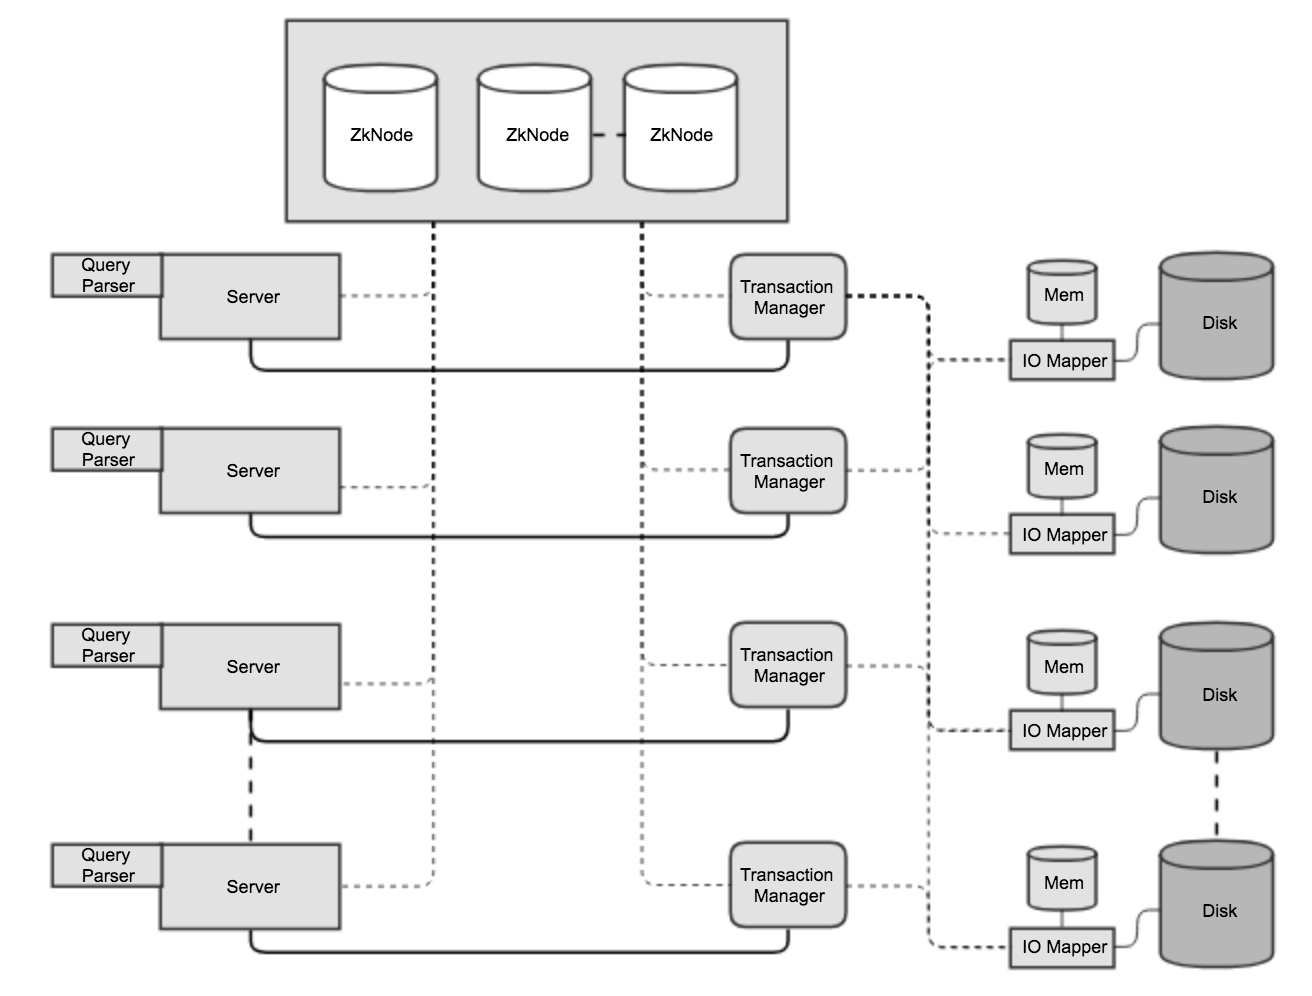
\includegraphics[width=0.5\textwidth]{comp.png}
\caption{Component Interaction Design}
\label{fig:comp}
\end{figure}
\begin{enumerate}
\item \textbf{Server}
The front facing servers make up the distributed gateway to access the database. Each server is a graph manipulation interface like Gremlin\cite{tinkerpop}. The servers in our implementation provide the same API end points as TinkerPop\cite{tinkerpop} graph interface over HTTP. The servers are completely stateless and each server only knows about the metadata cluster when it starts up from where it discovers and keeps track of all the storage backends. The API specification of the database server are described in the Section V1.B. The data accepted by the API server is encoded in JSON.\\
\item \textbf{Metadata Cluster}
The metadata cluster is made up of a bunch of Zookeeper nodes providing an fast ,in-memory and distributed key-value store for storing the metadata of the system like the list of storage backends, the location of partitions, replicas etc.\\
\item \textbf{Transaction Manager}
The transaction manager is responsible for figuring out the partition of the graph that needs to be read or manipulated and writing updates to vertices and edges in a consistent manner and replicating these writes to the replica partitions. We ensure that each partition of the graph is replicated on multiple storage backends where one of them acts as the primary at a time. We follow a chain replication mechanism where writes are first written onto the backup servers and then on the primary of that partition. The write operation is blocking and only returns once the write has propagated to the last backup server. Writes are serialized on the tail of the replication chain. We keep track of the servers responsible for hosting each partition on the metadata cluster. For ordering the writes on the replicas, we use the VersionIds returned from adding or manipulating metadata into the zookeeper. So, essentially the metadata cluster is our serialization point and all the replicas use this order to apply the write operations on their storage. \\
\item \textbf{I/O Mapper: }
The I/O Mapper is a storage abstraction with in memory indexing capabilities. It receives operations from the server and executes it on the local memory and storage. Each storage stores the vetices and edges of the partitions it is chosen to host along with their in-memory index.\\

\item \textbf{Partition Manager: }
The partition manager is basically the implementation of the partitioning logic of the graph. We first defined an interface to allocate a vertices and edges to a existing partition. We designed the interface to be utilized by the server while creating new componentd in the graph. We present evaluations based on two implementations of this interface as described in Section VI.C.
\end{enumerate}

\section{IMPLEMENTATION}
There are five central components to our implementation as described in Section V. We chose to use golang\cite{golang} for most of our code base mostly because of its concurrency features. To model graphs we first defined interfaces to abstract the raw data manipulation thereby providing handling of graph entities. Every entity in our database is made unique by assigning it a UUID generated using Google's UUID library. Our data model is based on the following design :
\begin{enumerate}
\item \textit{Graph} - A namespace for a set of vertices and edges. This permits multiple disjoint graphs to exist in different namespaces. This allows us to have a limited scope in queries. The namespace is identified using a UUID and can contain limited unstructured data encoded as a JSON string

\item \textit{Partition} - A partition is a logical grouping of components within a graph. This information is not persisted on storage and is never exposed to the end user. It is an entity purely for internal use and identified by a UUID. Each partition is a unit of replication that a certain number of storages can host 

\item \textit{Vertex} - A vertex is identified using the parent graphID and its own vertex UUID. Each vertex can hold a map of data where the key and value are modelled as strings. The string values can hold JSON encoded complex types but only the string keys and values at the top level are used for indexing and querying

\item \textit{Edge} - An edge is again identified using the parent graphID and its own edge UUID. Each edge has a label that defines the relation name, that is indexed and used for faster traversal. Additionally, each edge can contain a map of properties, just like a vertex
\end{enumerate}
Each exposed entity has a jsonEncoder defined which is invoked to package the entity for the HTTP API interface.
\subsection{Zookeeper Metadata Cluster} This component provides a centralized service for metadata management. It is a hierarchical key-value store, which provides a distributed configuration service, synchronization service, and naming registry. We use Zookeeper to provide the above functionalities. We use an ensemble of three sysnet VMs that are running the zookeeper service (version 3.4.12) at all times. We use Golang's zk\cite{go/zk} module to implement a client for the Zookeeper service. We developed graph-entity based abstractions over the APIs provided by the zk module to implement a zookeeper metadata mapper. The server and I/O mapper query into the Metadata Cluster using a metadata client, to obtain structural information about the graph. The methods exposed by this module are listed below :
\begin{enumerate}
\item \textbf{CreateVertexMetadata, CreateGraphMetadata, CreateEdgeMetadata, CreatePartitionMetadata, CreateBackendMetadata} - Creates znodes in the Zookeeper tree for the corresponding graph components. Backend znodes are ephemeral,sequential znodes that exist only as long as the backend is alive. All the other znodes are persistent and exist untill the corresponding delete calls are invoked
\item \textbf{DeleteVertexMetadata, DeleteEdgeMetadata} - Deletes znodes in the Zookeeper tree for the corresponding graph components. We let znodes corresponding to stale graph partitions persist in the tree for lack of time. We plan to optimize the tree structure and information retrieval in the future
\item \textbf{GetVertexLocation, GetEdgeLocation} - Return the partition that an edge/vertex belongs to along with the backend that houses that particular partition 
\item \textbf{SetVertexLocation, SetEdgeLocation} - Stores the new parition that an edge/vertex belongs to (after graph partitions are recomputed) in the corresponding znode
\item \textbf{GetAllBackends} - Returns the list of all backend IDs. Since znodes are associated with backends are ephemeral, this method returns the list of all live backends
\item \textbf{GetAllPartitions} - Returns all the partitions of a particular Graph shard 
\item\textbf{GetBackendsForPartition} - Returns all backends that house a particular partition
\item\textbf{GetBackendMetadata} - Returns the backend address associated with a particular Backend ID. We plan to expand the scope of this API to return any information stored at a backend znode, not just the backend address
\item \textbf{GetPartitionMetadata} - Returns the information stored at a partition znode. For now, the information stored at a partition znode is count of the number of elements that belong to a partition
\item\textbf{GetVertexMetadata} - Returns the information stored at a vertex znode. For now, the information stored at a vertex znode is the in-edge ID and the list of backends where the edge is stored
\item\textbf{GetEdgeInformation} - Returns the information stored at a vertex znode. For now, the information stored at a vertex znode is the destination vertex ID
\item \textbf{AddBackendToPartition} - Associates a backend's metadata with the metadata of the partition(s) that it houses. We set the first backend to be the primary by default
\item \textbf{IncrementElementCountMetadata} - Increments the count of the number of edges/vertices that belong to a particular partition of the graph. We update the count value by first getting the count value, adding 1 to it and then setting the count value back. We avoid concurrent count updates by leveraging version information. While setting the incremented count value, we make sure that we set the count value only if the version number on the znode is the same as the version number obtained while getting the count value
\item \textbf{DecrementElementCountMetadata} - Similar to IncrementCount. It is used to decrease count by 1
\end{enumerate}

The generated directory structure on the zookeeper nodes is shown in Fig. \ref{fig:zk_graph}. The grey nodes represent the ephemeral nodes that cease to exist once the respective backend connections are lost

\begin{figure}
 \centering
  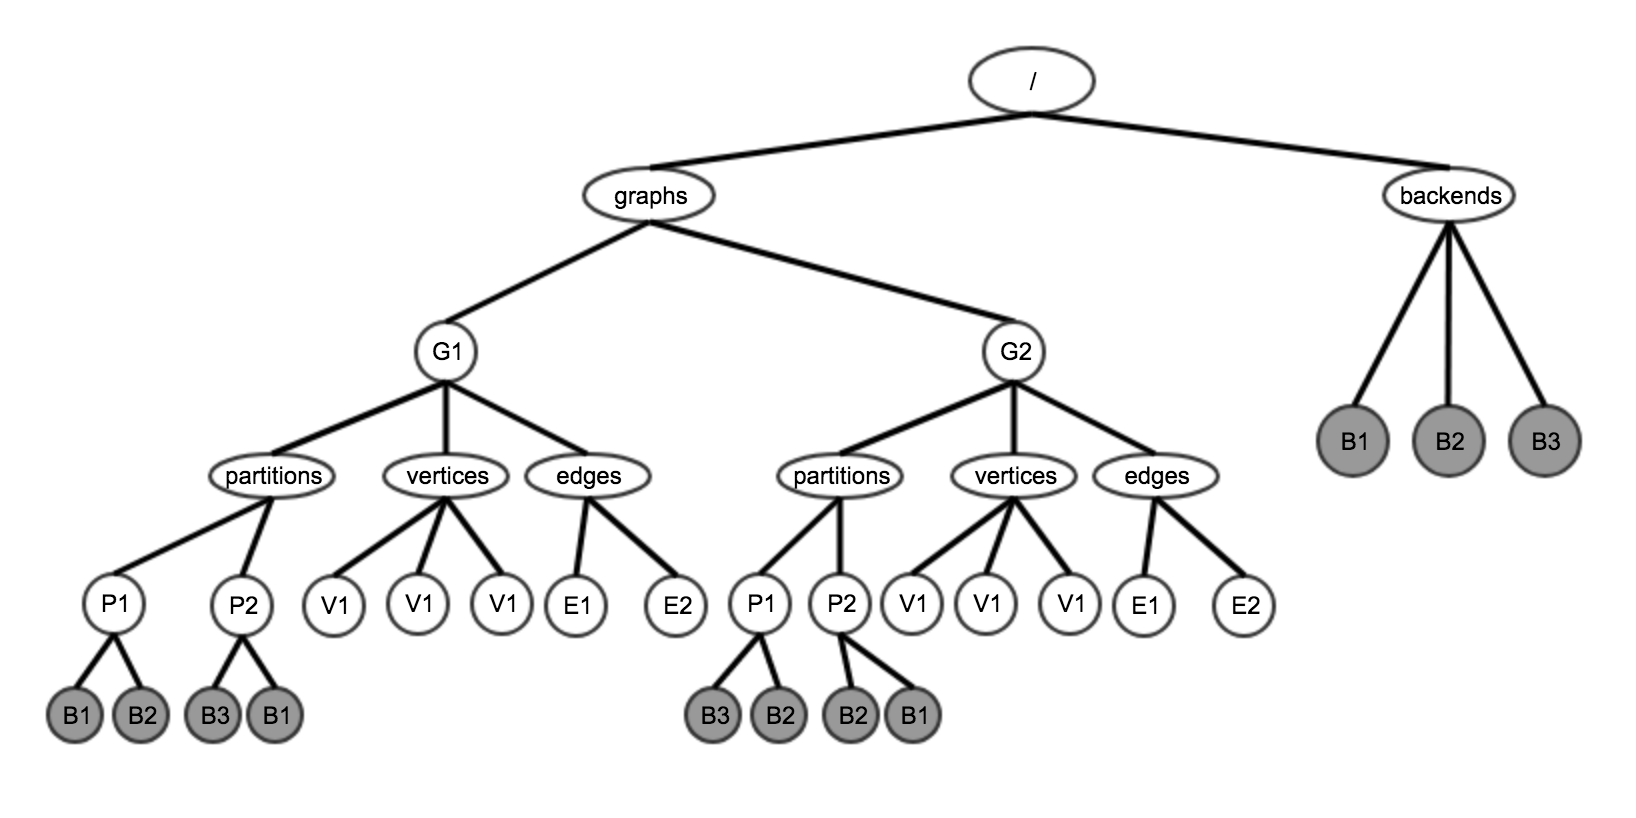
\includegraphics[width=0.5\textwidth]{zk_graph.png}
\caption{Zookeeper Directory Structure}
\label{fig:zk_graph}
\end{figure}
\subsection{Server} The server is responsible for receiving graph queries from the client and translating them to storage RPC calls, which in turn updates or fetches the corresponding elements from the in-memory key value store. The server provides a comprehensive set of APIs similar to Apache's TinkerPop\cite{tinkerpop} We use this to perforn complex graph traversals. The server also ensures consistency between metadata information in zookeeper and storage by ensuring that any action made on storage also results in an equivalent action on the metadata cluster. For example: A call to the "addvertex" API not only ensures addition of a new vertex, it also ensures that a znode is created in zookeeper for that vertex which contains information about the parition in which the vertex was stored. A list of these HTTP API's are given below:
\begin{enumerate}
\item \textbf{AddGraph}: Creates a new znode in zookeeper under \textit{/graphs} which indicates the creation of a new graph. The new znode is a UUID which denotes the unique ID given to the graph in the database. The graphUUID is returned which serves as a namespace for creating and querying new vertices and edges.
\item \textbf{GetGraphs}: Fetches a list of graph UUIDs by querying for the children of \textbf{/graphs}.
\item \textbf{AddVertex}: This API call requires a graph UUID and the vertex property set as input and it returns the UUID of the newly created vertex as ouput. All inputs and outputs are JSON encoded. We also create a znode at \textbf{/graphs/$<$graphid$>$/vertices/$<$vertexid$>$} that contains the partition ID under which the vertex is stored. We make sure the vertex is created on 3 backends before returning success.
\item \textbf{DeleteVertex}: Deletes the provided vertexID in the graph with the given graph ID. We first delete all the in-edges and out-edges of the vertex and only then do we delete the vertex itself. 
\item \textbf{GetVertex}: Gets all the vertex information for the provided vertexID.
\item \textbf{AddEdge}: Adds an edge between the two provided vertexIDs and returns an edgeID. We update zookeeper to store the created edge's ID and its backend information in the destination vertexID. This is so that we can directly query zookeeper to find the in-edges of any zookeeper. The edge is always stored in the same backends as the source vertexID 
\item \textbf{DeleteEdge}:  Deletes the provided edgeID in the graph with the given graph ID.
\item \textbf{GetEdge}: Gets all the vertex information for the provided edgeID.
\item \textbf{GetInEdges}: Get all the edge information for the in-edges associated with a vertex. We leverage the zookeeper metadata for a vertex to find its associated in-edges and their backends. We then make queries to the backends to fetch the edges' properties
\item \textbf{GetOutEdges}: Get all the edge information for the out-edges associated with a vertex. Since the out-edges are stored in the same backends as the source vertex, this API is easier to implement
\item \textbf{GetParentVertices}: Similar to GetInEdges, but returns the soruce vertex of the in-edges.
\item \textbf{GetChildVertices}: Similar to GetOutEdges, but returns the destination vertex of the out-edges.
\end{enumerate}

\subsection{Locator}
The locator service is responsible for identifying the partition within which a graph entity must be stored. It defines two methods: \textit{FindPartition} and \textit{RelocateElements}. The \textit{FindPartition} function is used to assign a partitionID to the vertex element that is newly being added into the graph. The \textit{RelocateElements} function is called whenever a new edge is added and is responsible for reassigning vertices to different partitions whenever a new edge is added.\\

We implement two types of locators: \textit{RandomLocator} and \textit{ConnectedComponentsLocator}. The \textit{RandomLocator} places vertices by randomly choosing a partition among available partitions. In case all partitions have reached maximum capacity, we create a new partition and the graph element to the new partition. The \textit{ConnectedComponentsLocator} relocates vertices that are connected so that they are in the same partition. Every time a new edge is added, we find the partition that contains the most number of neighbors of the source vertex and relocate the source vertex to that partition. New partitions are created whenever existing ones run out a predefined capacity.

\subsection{I/O Mapper Storage}

Storage is implemented as an RPC server that provides and interface to store, fetch and manipulate graph data. We call this interface an I/O Mapper. The main difference between this and a simple key value store is that this has in-memory index of the graph data it stores. Our implementation of the I/O Mapper uses a In-Memory key-value store to store indexes. The Diskstorage part was implemented using a memory mapped buffer which would easily be switched to a file with minimum effort. We leave aside the disk storage problem as designing the architecture to store local data is out of the purview of Distributed Systems. The I/O Mapper exposes RPCs to perform the following operations
\begin{enumerate}
\item \textbf{StoreVertex}, \textbf{StoreEdge} - These RPCs accepts the respective vertex or the edge object and store it in the local storage and also creates an index for faster access eliminating the need for fetching all the data during traversals. 
\item \textbf{GetVertexById}, \textbf{GetEdgeById} - These RPCs use the ID index to figure out the location of the entity and returns them.
\item \textbf{GetOutEdges} - This RPCs returns a complete set of edges that have a particular vertex as the source. This works as a complete set as we store the edge originating from a vertex on the same storage. Thus this call does not span across storages.
\item \textbf{GetInEdges} - This RPC is used by the server to accumulate the edges that have destination to a particular vertex. 
\item \textbf{RemoveVertex}, \textbf{RemoveEdge} - These RPCs accept the vertex/edge UUID respectively and delete them from the store. The call to \textbf{RemoveVertex} also ensures that all edges associated to the given vertex are deleted from the backend on which the query was issued on.
\item \textbf{UpdateProperties} - This RPC is used to update the property set for a vertex or an edge.
\item \textbf{RegisterToHostPartition} - This RPC is used to setup a watch on a partition. Whenever any backend dies, its ephemeral node in the partition subtree disappears and this RPC is used to watch for such events and trigger a replication of the partition information onto a new backend. 
\end{enumerate}

\section{Fault Tolerance Strategy}
As seen from the API structure, the storage is responsible for the health of the partition it hosts. Every time a storage is chosen by the Partition Manager to host a partition, it registers itself on to Zookeeper as an ephemeral node under the partition znode of the graph. This is done by each backend. So at any healthy partition, all the backends hosting that partition have a watch on that partition path. In case of a backend failure, the other backends hosting the same partitions will get triggers on the watch of the partition. When the watch gets triggered, the backend with the lexographically smallest backendId takes the responsibility of recovering the partition's replication status. It finds a new backend to replicate by querying the zookeeper and triggers replication on the new backend. At the completion of this stage, it finally calls the \textit{RegisterToHostPartition} RPC on the new backend to make it watch the partition like all others. This process is visualized in Fig. \ref{fig:fault} 


\begin{figure}
 \centering
  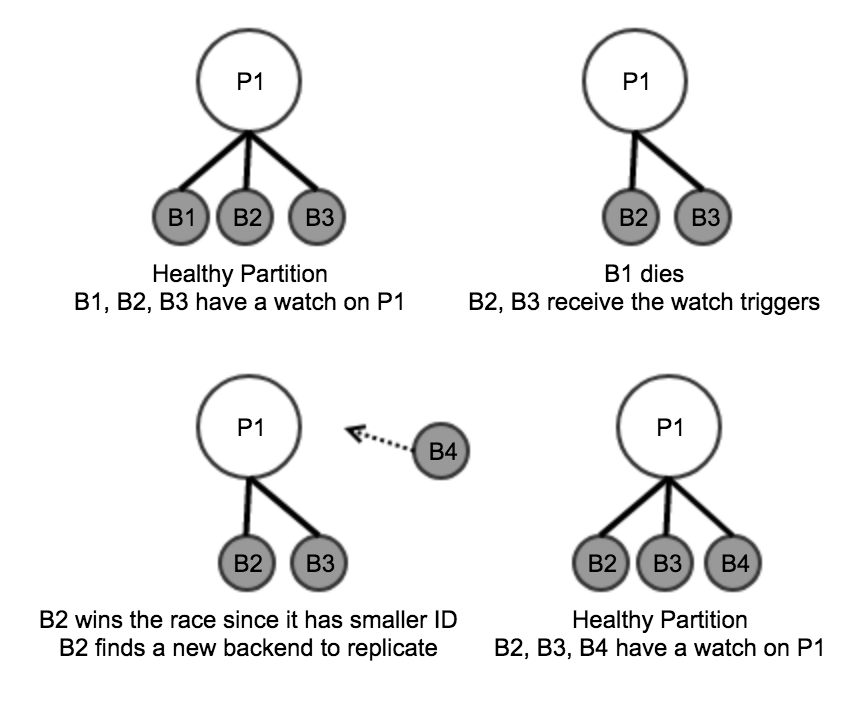
\includegraphics[width=0.5\textwidth]{fault.png}
\caption{Fault tolerance}
\label{fig:fault}
\end{figure}

\section{EVALUATION}
We evaluate our system to check if it matches the proposed promises of Scalability, Consistency and Fault-Tolerance. We failed storage backends to check fault tolerance and validated that there was no data loss. \\

For testing scalability, we made sure that the replication factor is a dynamic value that can be set in the Metadata store which the backends will honor. When the replication factor changes, we update the znode data on each partition that triggers a watch on the backends hosting that partition. The lead backend, which we define as the one with the lexographically smallest backendID, takes the responsibility of replicating its data onto a new backend. This happens even when a backend dies. We evaluated this promise by manually killing the backends and triggering the watches on the backend znodes. \\

Taking into account the time taken to design and implement our GraphDB, we steered clear of evaluating its performance against existing GraphDBs. Rather, we evaluated the performance of our system based on different vertex-placement strategies implemented in the Partition Manager component. In particular, we investigate if placing strongly connected vertices of a graph together achieves better performance than arbitrarily partitioning the vertices. As described in the implementation section our Partition Manager implemented two different logic of element placement. We evaluated both the implementations on common operations of graph databased as described below. \\

For the purpose of the evaluation we created a huge random graph of 10,000 vertices with a 0.25 probability of having an edge between any two randomly chosen vertices.\\


\begin{figure}
  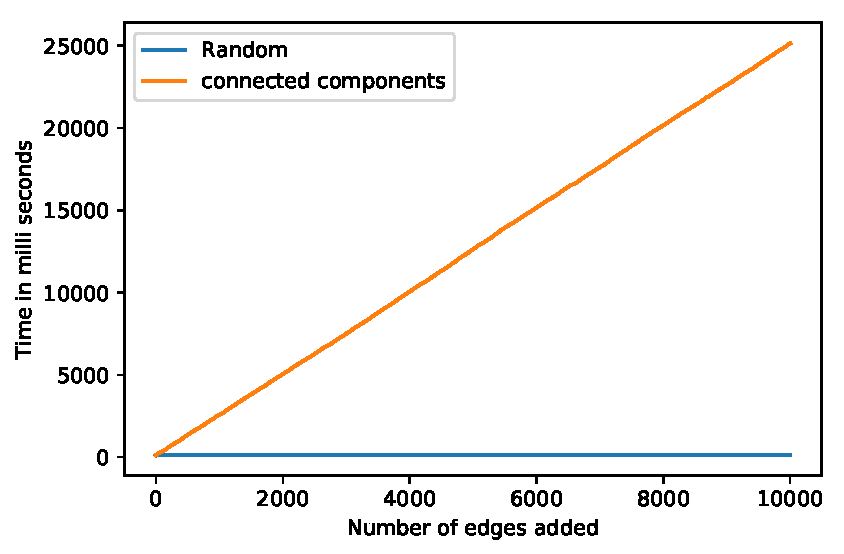
\includegraphics[width=\linewidth]{plot4.pdf}
  \caption{Variation of Insertion Latency with number of vertices and its connected components}
  \label{fig:plot4}
\end{figure}

\begin{figure}
  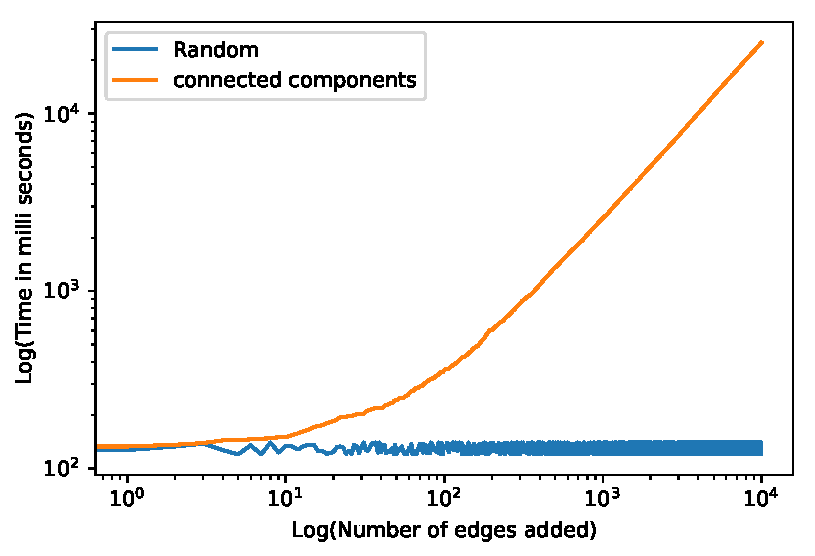
\includegraphics[width=\linewidth]{plot3.pdf}
  \caption{Log Plot of Variation of Insertion Latency with number of vertices and its connected components}
  \label{fig:plot3}
\end{figure}

\begin{figure}
  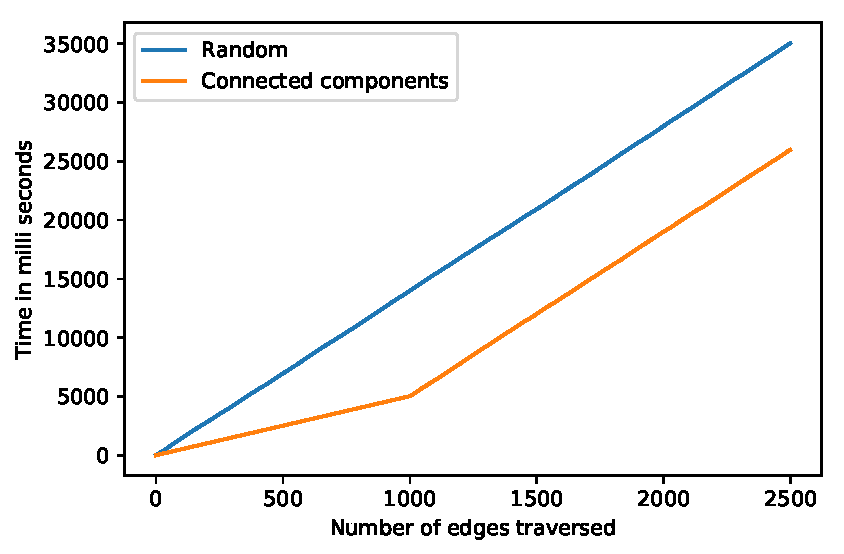
\includegraphics[width=\linewidth]{plot1.pdf}
  \caption{BFS Traversal}
  \label{fig:plot1}
\end{figure}

\begin{figure}
  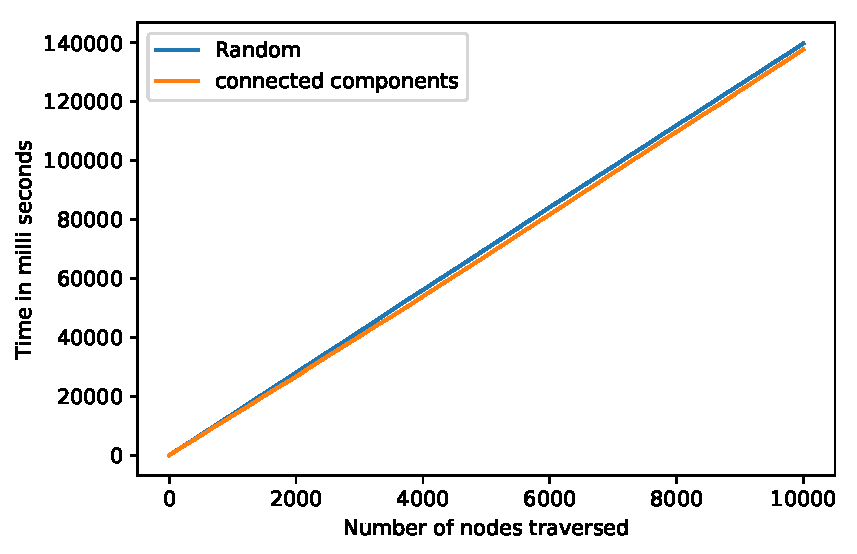
\includegraphics[width=\linewidth]{plot2.pdf}
  \caption{DFS Traversal}
  \label{fig:plot2}
\end{figure}





\begin{enumerate}
\item \textit{Insertion Latency}: We define insertion latency as the time required for the client to insert a new vertex into an existing graph and connecting it to the respective existing vertices using new edges. We predicted that the Common Component based vertex placement algorithm should add significant overhead to the insertion of new vertices and edges because we calculate the placement after querying other connected components of the graph and the connected components increase as the graphs grows bigger. We used the test graph to evaluate this overhead. We started from empty storage and added 10,000 vertices with the connecting edge in each iteration and recorded the time taken to insert the vertex. This raw data can be seen in Fig.\ref{fig:plot4}. We could not make out much difference in the linear scale so we decided to look at the Log scale of the time difference. As seen in Fig. \ref{fig:plot3}, insertion times increase significantly faster on the log scale.\\

\item \textit{BFS Traversal}: We define this evaluation metric as the time taken to traverse the graph using the breadth-first search algorithm which is used as a standard benchmark for all graph databases. Breadth-wise searches in graphs are popular and are often most time consuming. We used our test graph and evaluated the performance of BFS on graphs created using two different partitioning logics. As predicted by G-Store\cite{g-store}, we expected the connected component logic to perform better than the random. We observed the performance as seen in Fig. \ref{fig:plot1} 
\item \textit{DFS Traversal}: We define this evaluation metric as the time taken to traverse the graph from one random vertex to another random vertex using the Depth-first search algorithm. We see that in case of DFS, the difference in performance for the two different partitioning logics is almost neglibile. The results of this metric are seen in Fig. \ref{fig:plot2}

\end{enumerate}


\section{RESOURCES}
The complete software stack was tested and developed on the Lab VMs. We used servers vm170, vm171 and vm172 for all our work. 
\addtolength{\textheight}{-12cm}   % This command serves to balance the column lengths
                                  % on the last page of the document manually. It shortens
                                  % the textheight of the last page by a suitable amount.
                                  % This command does not take effect until the next page
                                  % so it should come on the page before the last. Make
                                  % sure that you do not shorten the textheight too much.

%%%%%%%%%%%%%%%%%%%%%%%%%%%%%%%%%%%%%%%%%%%%%%%%%%%%%%%%%%%%%%%%%%%%%%%%%%%%%%%%



%%%%%%%%%%%%%%%%%%%%%%%%%%%%%%%%%%%%%%%%%%%%%%%%%%%%%%%%%%%%%%%%%%%%%%%%%%%%%%%%



%%%%%%%%%%%%%%%%%%%%%%%%%%%%%%%%%%%%%%%%%%%%%%%%%%%%%%%%%%%%%%%%%%%%%%%%%%%%%%%%

%%%%%%%%%%%%%%%%%%%%%%%%%%%%%%%%%%%%%%%%%%%%%%%%%%%%%%%%%%%%%%%%%%%%%%%%%%%%%%%%

\bibliographystyle{plain}
\bibliography{references.bib}

\iffalse
\begin{thebibliography}{99}

\bibitem{c1} G. O. Young, ÒSynthetic structure of industrial plastics (Book style with paper title and editor),Ó 	in Plastics, 2nd ed. vol. 3, J. Peters, Ed.  New York: McGraw-Hill, 1964, pp. 15Ð64.
\bibitem{c2} W.-K. Chen, Linear Networks and Systems (Book style).	Belmont, CA: Wadsworth, 1993, pp. 123Ð135.
\bibitem{c3} H. Poor, An Introduction to Signal Detection and Estimation.   New York: Springer-Verlag, 1985, ch. 4.
\bibitem{c4} B. Smith, ÒAn approach to graphs of linear forms (Unpublished work style),Ó unpublished.
\bibitem{c5} E. H. Miller, ÒA note on reflector arrays (Periodical styleÑAccepted for publication),Ó IEEE Trans. Antennas Propagat., to be publised.
\bibitem{c6} J. Wang, ÒFundamentals of erbium-doped fiber amplifiers arrays (Periodical styleÑSubmitted for publication),Ó IEEE J. Quantum Electron., submitted for publication.
\bibitem{c7} C. J. Kaufman, Rocky Mountain Research Lab., Boulder, CO, private communication, May 1995.
\bibitem{c8} Y. Yorozu, M. Hirano, K. Oka, and Y. Tagawa, ÒElectron spectroscopy studies on magneto-optical media and plastic substrate interfaces(Translation Journals style),Ó IEEE Transl. J. Magn.Jpn., vol. 2, Aug. 1987, pp. 740Ð741 [Dig. 9th Annu. Conf. Magnetics Japan, 1982, p. 301].
\bibitem{c9} M. Young, The Techincal Writers Handbook.  Mill Valley, CA: University Science, 1989.
\bibitem{c10} J. U. Duncombe, ÒInfrared navigationÑPart I: An assessment of feasibility (Periodical style),Ó IEEE Trans. Electron Devices, vol. ED-11, pp. 34Ð39, Jan. 1959.
\bibitem{c11} S. Chen, B. Mulgrew, and P. M. Grant, ÒA clustering technique for digital communications channel equalization using radial basis function networks,Ó IEEE Trans. Neural Networks, vol. 4, pp. 570Ð578, July 1993.
\bibitem{c12} R. W. Lucky, ÒAutomatic equalization for digital communication,Ó Bell Syst. Tech. J., vol. 44, no. 4, pp. 547Ð588, Apr. 1965.
\bibitem{c13} S. P. Bingulac, ÒOn the compatibility of adaptive controllers (Published Conference Proceedings style),Ó in Proc. 4th Annu. Allerton Conf. Circuits and Systems Theory, New York, 1994, pp. 8Ð16.
\bibitem{c14} G. R. Faulhaber, ÒDesign of service systems with priority reservation,Ó in Conf. Rec. 1995 IEEE Int. Conf. Communications, pp. 3Ð8.
\bibitem{c15} W. D. Doyle, ÒMagnetization reversal in films with biaxial anisotropy,Ó in 1987 Proc. INTERMAG Conf., pp. 2.2-1Ð2.2-6.
\bibitem{c16} G. W. Juette and L. E. Zeffanella, ÒRadio noise currents n short sections on bundle conductors (Presented Conference Paper style),Ó presented at the IEEE Summer power Meeting, Dallas, TX, June 22Ð27, 1990, Paper 90 SM 690-0 PWRS.
\bibitem{c17} J. G. Kreifeldt, ÒAn analysis of surface-detected EMG as an amplitude-modulated noise,Ó presented at the 1989 Int. Conf. Medicine and Biological Engineering, Chicago, IL.
\bibitem{c18} J. Williams, ÒNarrow-band analyzer (Thesis or Dissertation style),Ó Ph.D. dissertation, Dept. Elect. Eng., Harvard Univ., Cambridge, MA, 1993. 
\bibitem{c19} N. Kawasaki, ÒParametric study of thermal and chemical nonequilibrium nozzle flow,Ó M.S. thesis, Dept. Electron. Eng., Osaka Univ., Osaka, Japan, 1993.
\bibitem{c20} J. P. Wilkinson, ÒNonlinear resonant circuit devices (Patent style),Ó U.S. Patent 3 624 12, July 16, 1990. 
\bibitem{c21} https://linux.die.net/man/1/qperf





\end{thebibliography}
\fi



\end{document}
